\section{Results}

\subsection{Cross sections and ratios}

The flux averaged cross section and ratio values measured in the FHC
and RHC samples are extracted from the flux, the number of targets,
MC efficiencies and MC background estimates. The input parameters
are given in Table \ref{tab:input to final cross sections} and the
results for the restricted (full) phase space selections are given in
Tables \ref{tab:Restricted-phase-space-cross_sections}( \ref{tab:Full-phase-space_cross_sections}).
The systematic errors in Table \ref{tab:Restricted-phase-space-cross_sections}
are determined by adding in quadrature the errors in 
Tables III, IV and V. For example the fractional R error,
taken from the three Tables, is 4\% and this yields 0.015
for the absolute systematic R error in Table VII. 

In Table \ref{tab:input to final cross sections},
for the restricted phase space results,
the input parameters
include the $\nu_\mu$($\overline\nu_\mu$) fluxes normalized to PoT in the FHC(RHC) samples. 
The number of nucleon targets is given for both the data and MC
which slightly differed. The number of reconstructed MC events is
given scaled to the equivalent data PoT. The data/MC generated corrected
events are defined as the reconstructed data/MC generated events,
minus the MC background and divided by the MC CCINC efficiencies.
%This is done for both the restricted and the full phase space selected
%samples.

In Table \ref{tab:Full-phase-space_cross_sections}, the full phase
space results are extrapolated
by scaling the restricted values in Table \ref{tab:input to final cross sections}
by the ratio of the total to restricted cross sections as predicted by the
NEUT MC generator.  The single errors combine the
statistical and systematic errors, which included 
model uncertainties on the assumed values of
$M_A^{QE}$ and the 2p2h $C^{12}$  and $O^{16}$ parameters in the scaling factor.
The errors
on the $\nu_\mu$ and \nubar cross sections due to these parameter
uncertainties
were assumed to be totally uncorrelated leading to a conservative
estimate of the systematic errors on the full phase space
ratio of cross sections.

The cross section calculations use Eqn.(\ref{eq:Analysis:6-1})
and the ratio $R(\nu,\overline{\nu})$ is obtained from Eqn.(\ref{eq:Analysis:7-1}) where
we note the number of targets drops out. 
%We include the additional
%quantities, sum and difference of cross sections and the ratio of
%the difference over the sum of cross sections which forms an asymmetry
%denoted as $A$. 
We find $\approx 10\%$
systematic cross section
errors whereas the ratio of cross sections $R(\nu,\overline{\nu})$ error
%and $A(\nu,\overline{\nu})$ 
has a factor $\times2$
smaller values of $4.0\%$ 
%{\color{blue}\st{($5.2\%$)} }
errors for the restricted 
%{\color{blue}\st{(full)} }
phase space.
These systematic errors are mainly due to the flux uncertainties 
on the flux prediction which
have strong correlations between neutrino and antineutrino fluxes
which largely cancel in the ratio.  %{\color{blue}
The flux predictions for neutrino mode and antineutrino mode are correlated through measurements that are used as inputs to the flux calculation.  These measurements include the proton beam current measurement, the measurement of the primary proton interaction rate by NA61/SHINE, and the measurement of secondary particle interaction rates by other hadron interaction experiments.
The measured ratio of rates  $r(\nu,\overline{\nu})$  
given in Eqn.(\ref{eq:Analysis:7-2}) represents the ratio
of $\nu_\mu$ and $\bar\nu_\mu$ event rates which depends on the integrated
FHC and RHC flux and so its value depends on the particular experiment and data taking periods.
The event rate ratio $r(\nu,\overline{\nu})$  
fractional systematic uncertainty is the same as 
cross section ratio
$R(\nu,\overline{\nu})$, except
it does not include the flux errors given in Table \ref{tab:BeamFluxSummary}. The fractional 
systematic errors are $1.92\%$ 
%{\color{blue}\st{($3.6\%$) } }
for the restricted 
%{\color{blue}\st{(full)}}  
phase space selections.

%{\color {red}We summarize the complete systematic errors in Table XX. [to be added]}

\begin{table*}
\caption{\label{tab:input to final cross sections}
Tabulation of flux, targets,
and data/MC events used in the cross section calculations.
The data corrected values are background
subtracted and divided by the MC efficiency.
}
\begin{tabular}{lccc}
%\toprule 
\hline
\hline
Inputs for Cross Sections & Units & RHC $\overline{\nu}$ mode & FHC $\nu$ mode \tabularnewline
\midrule 
Integrated flux  & {[}cm$^{2}$/10$^{21}$ PoT{]}  & 1.477$\times10^{13}$  & 1.823$\times10^{13}$\tabularnewline
Number of targets (data)  & {[}Nucleons{]}  & 3.147$\times10^{30}$  & 3.147$\times10^{30}$ \tabularnewline
Number of targets (MC)  & {[}Nucleons{]}  & 3.119$\times10^{30}$  & 3.119$\times10^{30}$ \tabularnewline
\midrule 
Number of data/MC events (restricted PS) & {[}Events{]} & 1,498/1,634 & 14,398/15,284
%& 1,860/1,945 & 19,090/19,532
 \tabularnewline
Data corrected (restricted PS) & {[}Events/10$^{21}$ PoT{]}   & 41,821$\pm$1,334 & 138,576$\pm$1,249
%& 42,119$\pm$1,211  & 141,400$\pm$1,128 
\tabularnewline
%MC Generated corrected{*} (restricted PS) & {[}Events/10$^{21}$ PoT{]}  & 43,886$\pm$285  & 142,463$\pm$391\tabularnewline
%\midrule
%Number of data/MC events (full PS) & {[}Events{]} & 1,869/1,953 & 19,259/19,566\tabularnewline
%Data corrected (full PS) & {[}Events/10$^{21}$ PoT{]}  & 86134$\pm$2474 & 425251$\pm$3355\tabularnewline
%MC Generatead corrected (full PS) & {[}Events/10$^{21}$ PoT{]}  & 89911$\pm$546 & 428335$\pm$1063\tabularnewline
%\bottomrule
\hline
\hline
\end{tabular}
\end{table*}


\begin{table*}
\caption{\label{tab:Restricted-phase-space-cross_sections} Restricted phase
space cross section and ratio final results.}

\begin{tabular}{crcl}
\hline
\hline 
\multicolumn{4}{c}{Cross Sections {[}$\times10^{-39}$cm$^{2}$/nucleon
{]} }\tabularnewline
%{\color{blue}
\hline 
$\sigma\left(\overline{\nu}\right)$  & 0.900  & $\pm$0.029 (stat.)  & $\pm0.088$ (syst.) \tabularnewline
$\sigma\left(\nu\right)$ & 2.41  & $\pm$0.022 (stat.)  & $\pm0.231$ (syst.) \tabularnewline
%$\sigma(\nu)-\sigma($$\overline{\nu}$$)$  

$\Delta(\nu,\overline\nu)$   & 1.512  & $\pm$0.036 (stat.)  & $\pm$0.152 (syst.) \tabularnewline
%$\sigma(\nu)+\sigma($$\overline{\nu}$$)$  
$\Sigma(\nu,\overline\nu)$    & 3.311  & $\pm$0.036 (stat.)  & $\pm$0.318 (syst.) \tabularnewline
\hline 
\multicolumn{4}{c}{Ratios}\tabularnewline
\hline 
%$\sigma\left(\overline{\nu}\right)$/$\sigma\left(\nu\right)$ 
$R(\nu,\overline\nu)$  & 0.373  & $\pm$0.012 (stat.)  & $\pm$0.015 (syst.) \tabularnewline
%$(\sigma(\nu)-\sigma($$\overline{\nu}$$))/(\sigma(\nu)+\sigma($$\overline{\nu}$$))$  
$A(\nu,\overline\nu)$  & 0.457  & $\pm$0.012 (stat.)  & $\pm$0.17 (syst.) 
%}
\tabularnewline
\hline
\hline 
\end{tabular}
\end{table*}

\begin{table*}
\caption{\label{tab:Full-phase-space_cross_sections}
Full phase space cross sections and ratio results extrapolated from restricted phase space measurements.}
\begin{tabular}{crcl}
\hline
\hline 
\multicolumn{3}{c}
{%Full Phase Space 
Cross Sections {[}$\times10^{-39}$cm$^{2}$/nucleon{]} }\tabularnewline
\hline 
$\sigma\left(\overline{\nu}\right)$ & 1.71 & $\pm$0.29 (stat.+syst.)    \tabularnewline
$\sigma\left(\nu\right)$ & 7.07 & $\pm$1.20 (stat.+syst.)   \tabularnewline
\hline 
\multicolumn{3}{c}{Ratios}\tabularnewline
\hline 
%$\sigma\left(\overline{\nu}\right)$/$\sigma\left(\nu\right)$ 
$R(\nu,\overline\nu)$  & 0.242 & $\pm$0.058 (stat.+syst.)    \tabularnewline
\hline
\hline 
\end{tabular}

\end{table*}

\begin{figure*}
%\includegraphics[scale=0.8]{generate-full_CCinc}
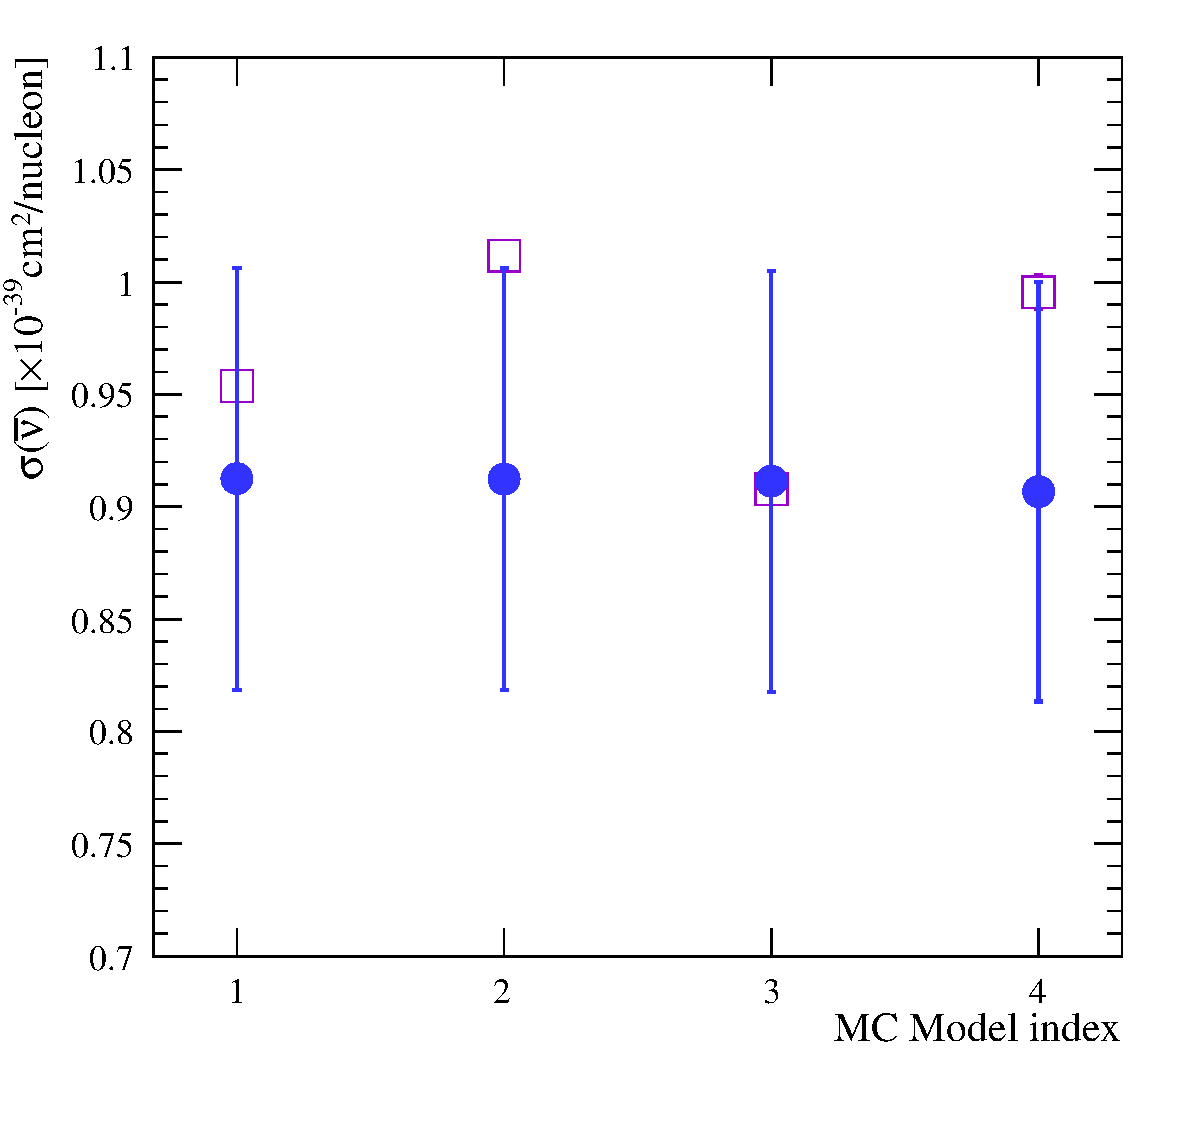
\includegraphics[scale=0.25]{MCComparisonAntiNu}
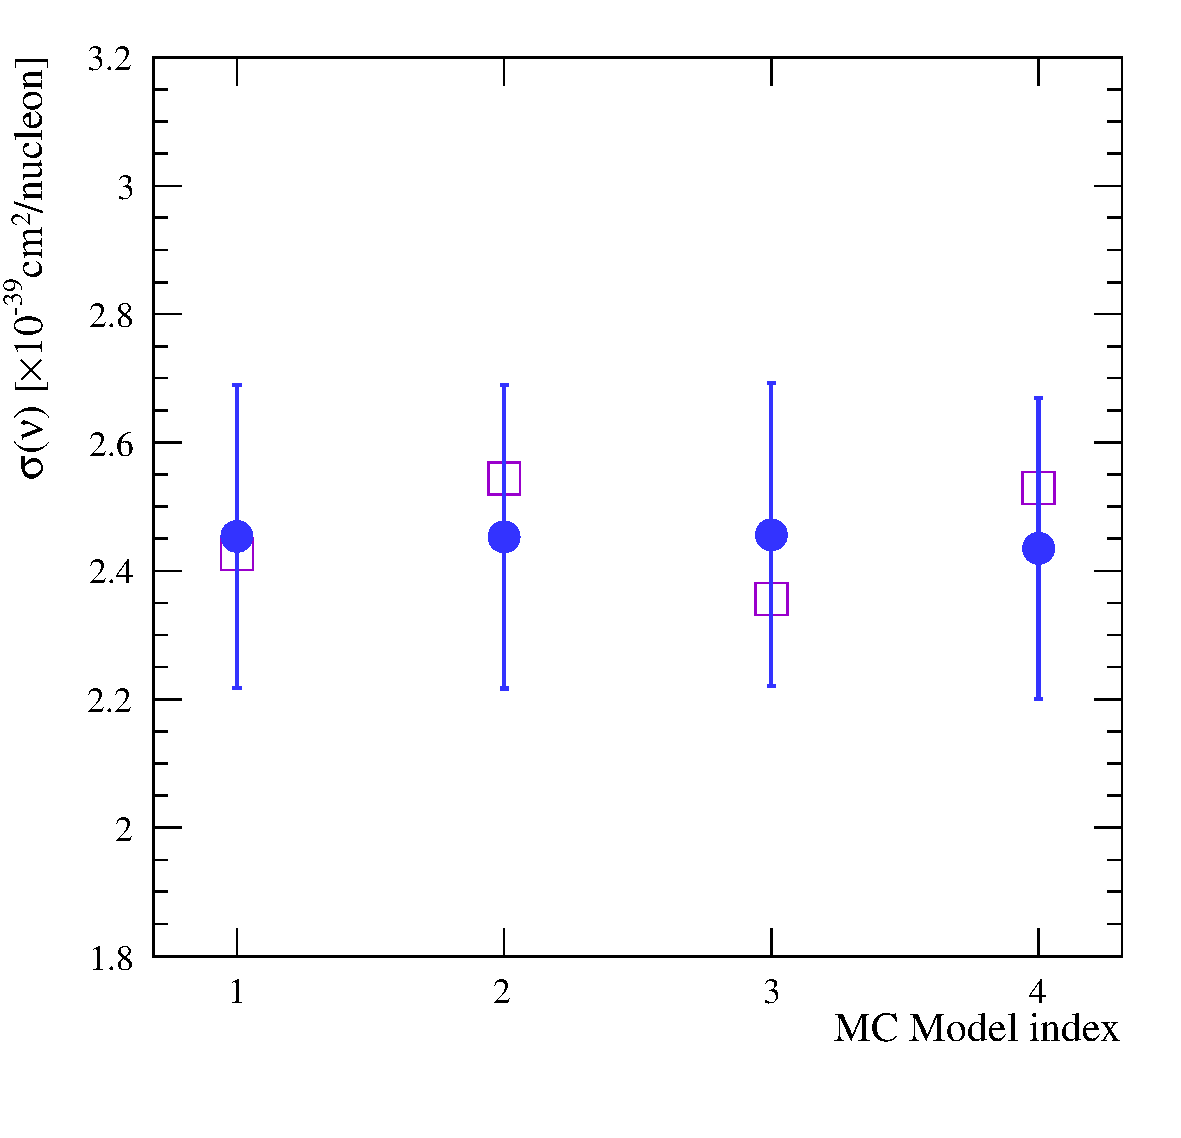
\includegraphics[scale=0.25]{MCComparisonNu}
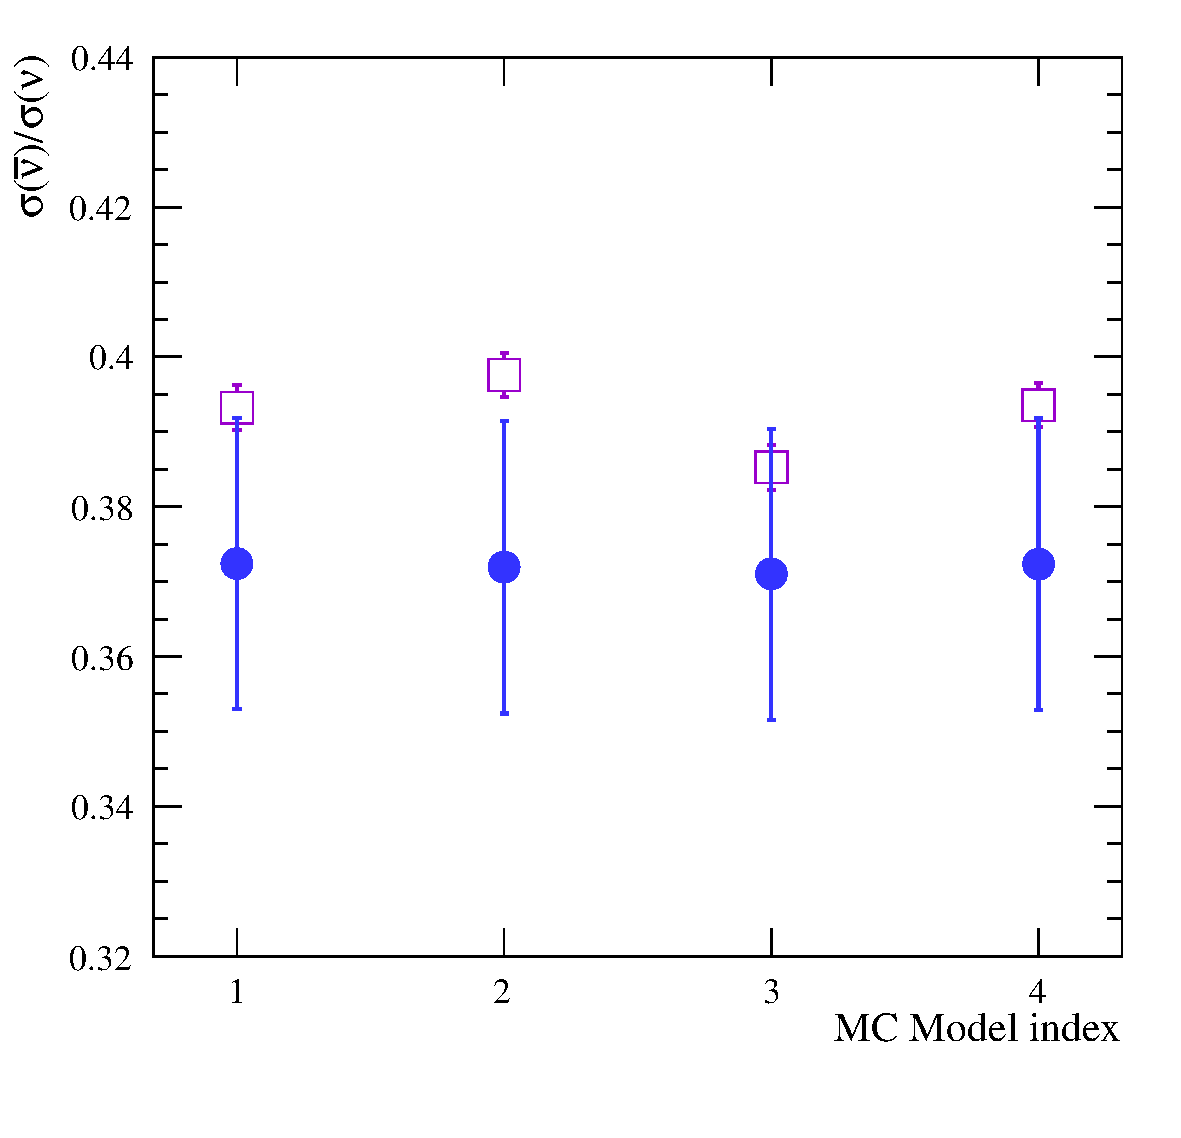
\includegraphics[scale=0.25]{MCComparisonR}

\caption{\label{fig:2p2h-compare-1}  
Comparison of MC model 1-4 predictions, open squares with no errors bars, to data results, 
solid circles with error bars, in measurements 
of cross sections $\sigma(\bar\nu_\mu)$ [Left] 
and $\sigma(\nu_\mu)$ [Middle]  
and the $R$ ratio $\sigma(\bar\nu_\mu) / \sigma(\nu_\mu)$ [Right].
}
\end{figure*}

\begin{figure*}
%\includegraphics[scale=0.8]{generate-full_CCinc}
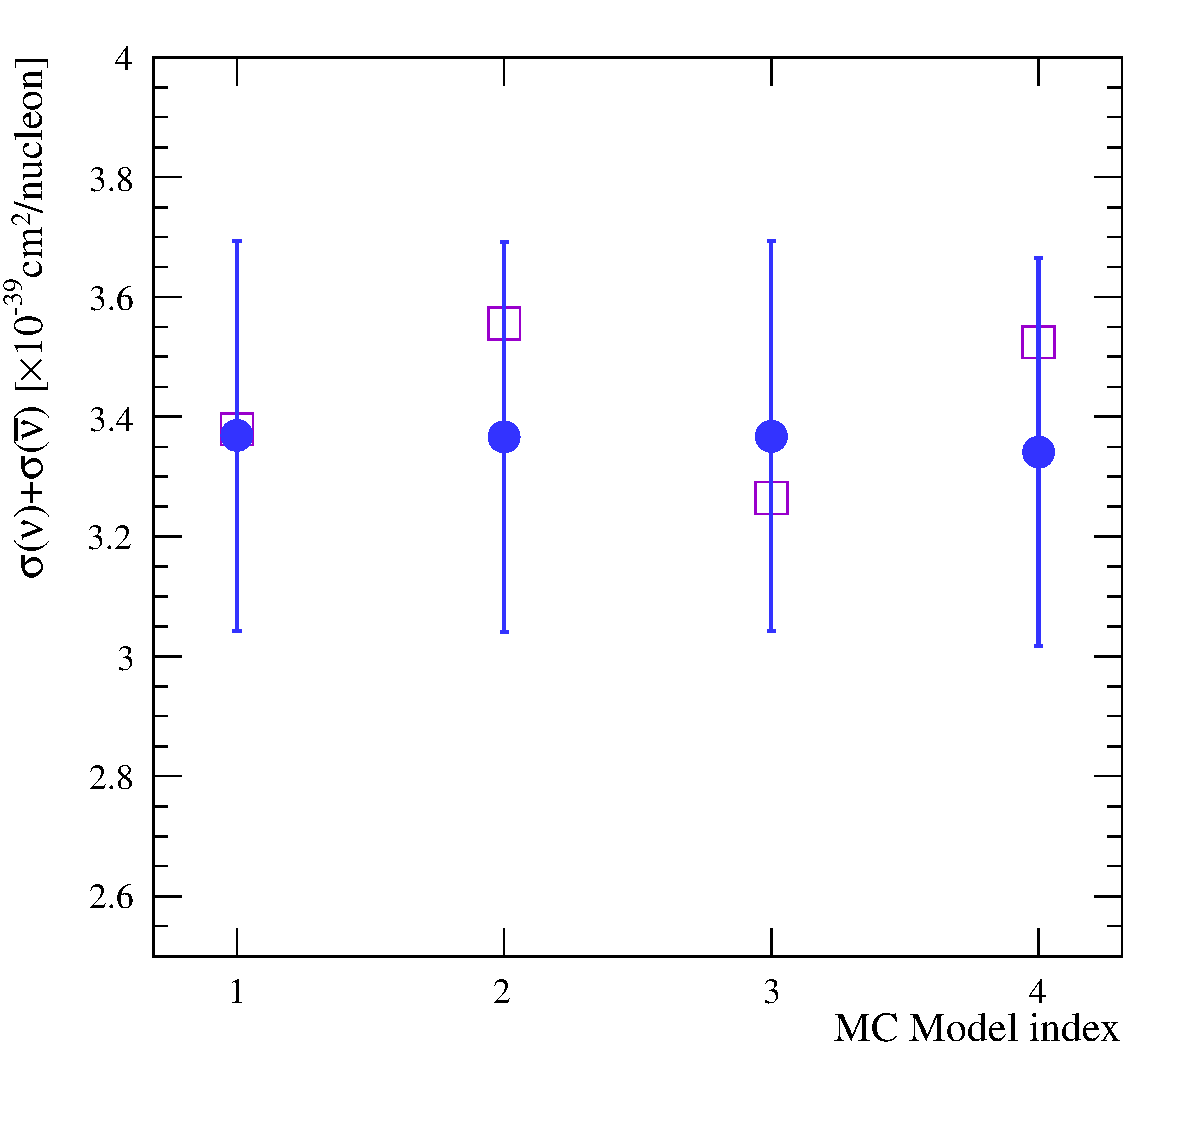
\includegraphics[scale=0.25]{MCComparisonSum}
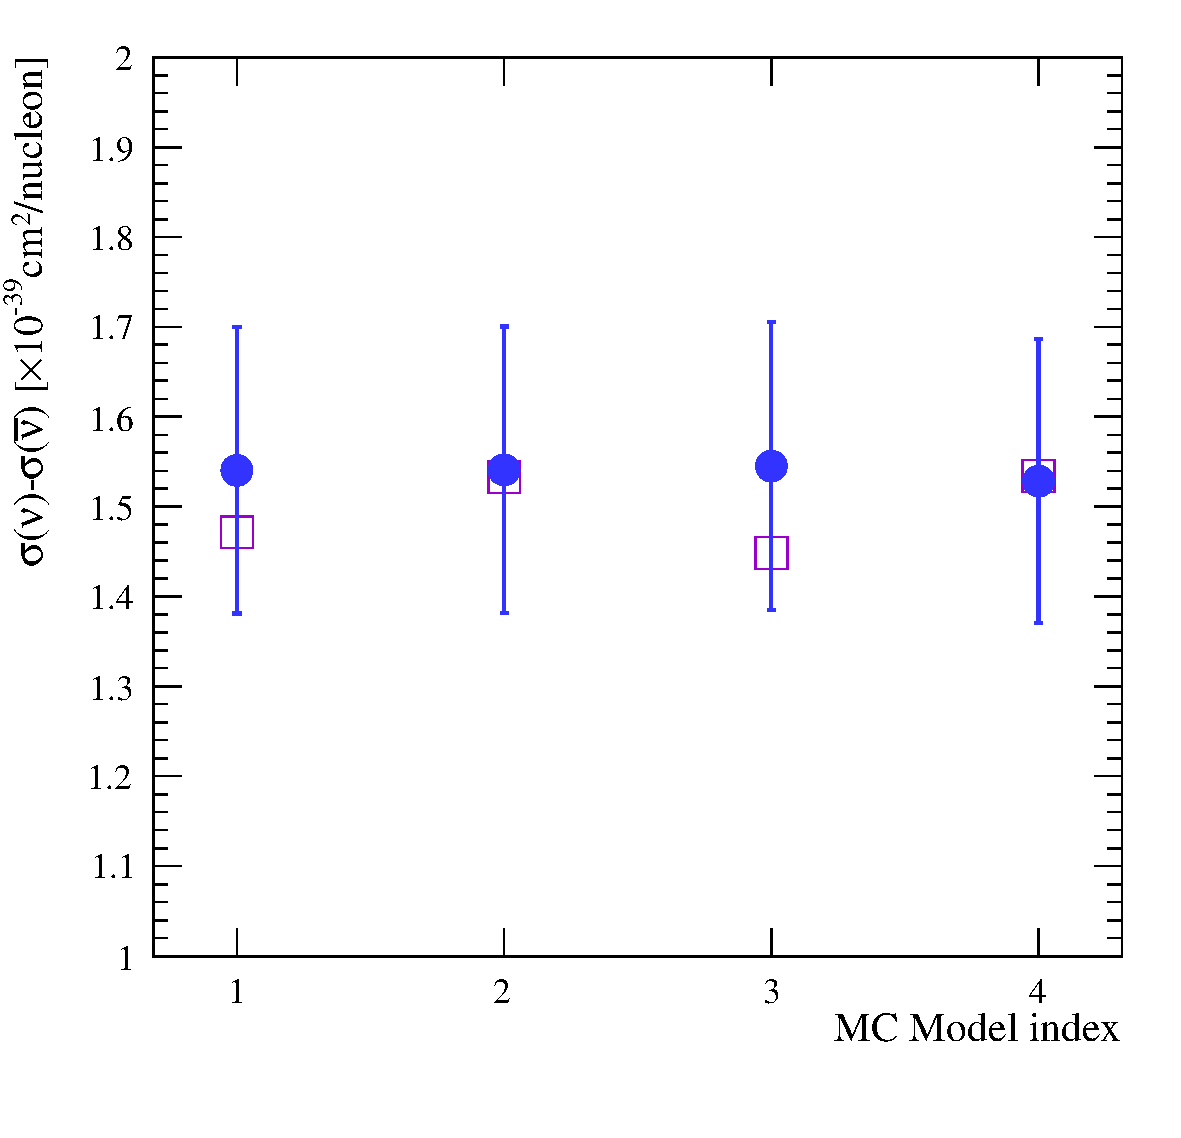
\includegraphics[scale=0.25]{MCComparisonSub}
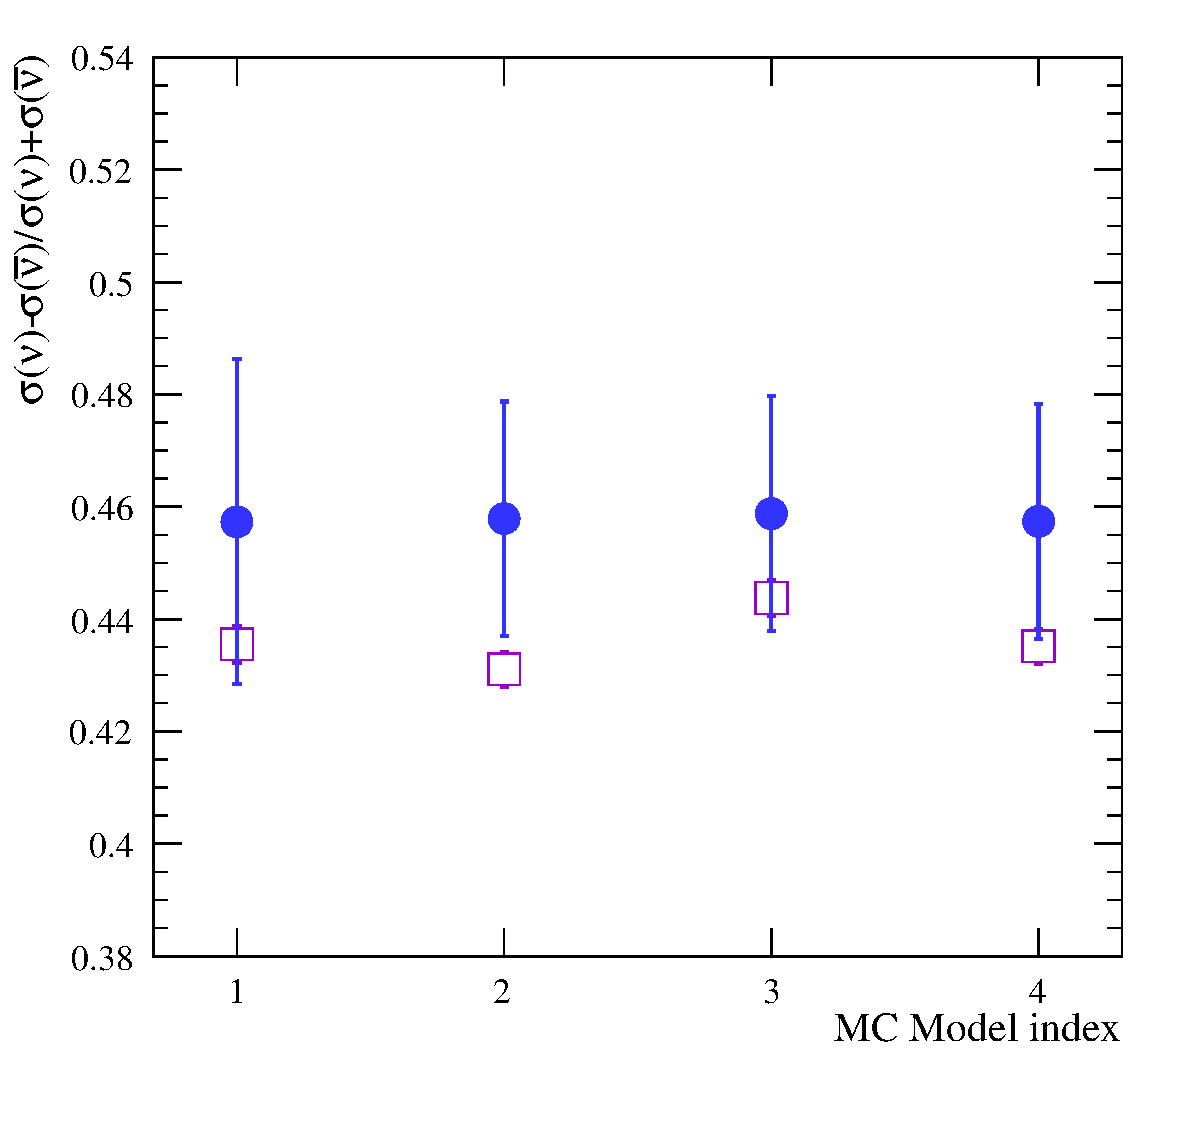
\includegraphics[scale=0.25]{MCComparisonAsy}

\caption{\label{fig:2p2h-compare-2} 
 Comparison of MC model 1-4 predictions, open squares with no errors bars, to data results, 
solid circles with error bars, in measurements 
of the cross section sum $\Sigma=\sigma(\nu_\mu)+\sigma(\bar\nu_\mu)$ [Left], 
difference $\Delta=\sigma(\nu_\mu)-\sigma(\bar\nu_\mu)$ [Middle]  
and
asymmetry $A=( \sigma(\nu_\mu)-\sigma(\bar\nu_\mu) )$/$( \sigma(\nu_\mu)+\sigma(\bar\nu_\mu) )$ [Right].
}
\end{figure*}

\begin{table*}
\caption{
\label{tab:show-model3} 
The numerical values of model 3 predictions and 
the corresponding measurements shown in Figs. \ref{fig:2p2h-compare-1} 
 and \ref{fig:2p2h-compare-2}.
}

%\resizebox{\columnwidth}{!}{
%\begin{ruledtabular}
\begin{tabular}{lcccccc}
\hline
\hline
Model 3 &  $\sigma(\overline{\nu})$ & $\sigma(\nu)$ & $\Delta(\nu,\overline{\nu})$ & $\Sigma(\nu,\overline{\nu})$ & $R(\nu,\overline{\nu})$ & $A(\nu,\overline{\nu})$ \\
\hline
MC predictions   & $0.908$ & $2.36$ & $1.45$ & $3.26$ & $0.385$ & $0.444$ \\
Measurements & $0.911\pm0.094$ & $2.45\pm0.24$ & $1.55\pm0.16$ & $3.37\pm0.33$ & $0.371\pm0.019$ & $0.459\pm0.021$ \\

%  & $\pm0.38$ & $\pm0.33$ & $\pm0.05$ & $\pm0.05$ & $\pm0.34$ & $\pm0.30$ \\
\hline
\hline
\end{tabular}
%\end{ruledtabular}
%}
\end{table*}


%\begin{table*}
%\caption{\label{tab:compare models}
%{\color{blue} Predicted  cross sections and ratios for different models. See text for model 1-4
%descriptions. The errors are only statistical from the generated events} }

%\centering
%\begin{tabular}{ccccccc}
%\toprule
%\hline
%Model &  $\sigma(\bar\nu)$ &  $\sigma(\nu)$ & $\sigma(\nu)-\sigma(\bar\nu)$ & $\sigma(\nu)+\sigma(\bar\nu)$  & $\sigma(\bar\nu) /  \sigma(\nu)$ & $(\sigma(\nu)-\sigma(\bar\nu))/(\sigma(\nu)+\sigma(\bar\nu))$ \\
%1 & $0.9539\pm0.0032$ & $2.426\pm0.0032$ & $1.4718\pm0.0047$ & $3.3796\pm0.0047$ & $0.39323\pm0.00142$ & $0.43551\pm0.00152$ \\
%2 & $1.0117\pm0.0032$ & $2.544\pm0.0036$ & $1.5328\pm0.0048$ & $3.5562\pm0.0048$ & $0.3976\pm0.00139$ & $0.43102\pm0.00148$ \\
%3 & $0.9079\pm0.0031$ & $2.356\pm0.0035$ & $1.4486\pm0.0046$ & $3.2643\pm0.0046$ & $0.38527\pm0.00142$ & $0.44376\pm0.00155$ \\
%4 & $0.9955\pm0.0032$ & $2.529\pm0.0036$ & $1.5339\pm0.0048$ & $3.5249\pm0.0048$ & $0.39357\pm0.00139$ & $0.43516\pm0.00149$ \\
%\hline
%\bottomrule
%\end{tabular}
%\end{table*}

%\begin{table*}
%\caption{\label{tab:compare data results}
%{\color{blue} Observed from data the cross sections and ratios using efficiencies from different models. 
%The results have very little changes between the different models 1-4.} }

%\centering
%\begin{tabular}{ccccccc}
%\toprule
%\hline
%Model &  $\sigma(\bar\nu)$ &  $\sigma(\nu)$ & $\sigma(\nu)-\sigma(\bar\nu)$ & $\sigma(\nu)+\sigma(\bar\nu)$  & $\sigma(\bar\nu) /  \sigma(\nu)$ & $(\sigma(\nu)-\sigma(\bar\nu))/%(\sigma(\nu)+\sigma(\bar\nu))$ \\

%1 & $0.9125\pm0.0939$ & $2.4540\pm0.2361$ & $1.5411\pm0.1596$ & $3.3660\pm0.03255$ & $0.37189\pm0.01949$ & $0.45784\pm0.02091$ \\
%2 & $0.9106\pm0.0937$ & $2.517\pm0.2359$ & $1.5411\pm0.1600$ & $3.3623\pm0.3252$ & $0.37143\pm0.01970$ & $0.45834\pm0.02093$ \\
%3 & $0.9113\pm0.0938$ & $2.4563\pm0.2364$ & $1.5450\pm0.1600$ & $3.3676\pm0.3257$ & $0.37100\pm0.01945$ & $0.45879\pm0.02095$ \\
%4 & $0.9066\pm0.0933$ & $2.4348\pm0.2343$ & $1.528\pm0.1583$ & $3.3414\pm0.3232$ & $0.37235\pm0.01953$ & $0.45735\pm0.02091$ \\

%\hline
%\bottomrule
%\end{tabular}
%\end{table*}
 
\subsection{Discussion of results}

In this section we discuss how our results compare with NEUT predictions, previous measurements,
the impact on future CPV measurements and the multinucleon effects that can modify neutrino
cross sections.

We observe close agreement between the numbers of data events
and the NEUT MC generated events in both the unrestricted and restricted
phase space selected events. Using Table \ref{tab:input to final cross sections},
the data to MC ratios for the restricted phase space selection
for the FHC/RHC modes are 94.2\%/91.7\%.
%and the full PS selection ratios are again 99\% and 96\%, respectively.
%The full PS neutrino cross section in Table \ref{tab:Full-phase-space_cross_sections} agrees quite well
%with the previous CCinc measurement\citep{t2k-carbon-ccinc} in the ND280 FGD sub-detector.
%The fractional uncertainties of the restricted PS selected \nuandnubar cross 
%sections and the $R$ ratio are 10\%, 9\% and
%5\%, respectively. 
%{\color{red}As discussed in the previous section, the smaller fractional errors on 
%the ratio compared to the fractional errors on the absolute cross section 
%are due the correlated flux errors this is caused by Mark Hariz explanation.}


%Due to the cancellation of the flux errors, the fractional 
%systematic error on the ratio is decreased
%by a factor two smaller relative to the absolute cross section errors. 

We can compare our neutrino result to previous 
T2K publications that used the FGD sub-detector with a scintillator target.
The previous T2K flux averaged
CCINC \citep{t2k-carbon-ccinc} was 
 $(6.91\pm0.13{\rm (stat.)}\pm0.84{\rm (syst.)}) \times 10^{-39}$cm$^2$  per nucleon
and this is within systematic errors to our full phase space measurement
 %of $(7.40\pm0.058{\rm (stat.)}\pm0.656{\rm (syst.)}) \times 10^{-39}$cm$^2$  per nucleon
in Table \ref{tab:Full-phase-space_cross_sections}.
The published T2K CCQE \citep{t2k-cceq} and 
events of the charged current process that has no pions (CC0$\pi$) \citep{cc0pi}
flux averaged cross sections per nucleon are
$(3.83\pm0.55) \times 10^{-39}$cm$^2$ 
and
$(4.17\pm0.05\pm0.47) \times 10^{-39}$cm$^2$, respectively. 
In the context of the NEUT model, the CCINC results presented here are 
compatible with the CCQE and CC0pi results from these prior publications.
%{\color{green}Using the fractions neutrino CCQE and CC0$\pi$ fractions from NEUT, our estimated
%CCQE and CC0$\pi$ cross sections/$10^{-39}$cm$^2$ 
%based on our neutrino CCINC sample in Table VIII yields
%3.38 and 4.23, respectively, which are in good agreement with previous T2K publications.} 
%{\color{blue}
%$(3.88\pm.57) \times 10^{-39}$cm$^2$ 
%and
%$(4.23\pm.72) \times 10^{-39}$cm$^2$, respectively.} 
%Using our full phase space CCinc neutrino cross section 
%$(7.40\pm0.058{\rm (stat.)}\pm0.656{\rm (syst.)}) \times 10^{-39}$cm$^2$  per nucleon
%we can indirectly estimate the CCQE component using 
%Table \ref{tab:The-fractional-distribution-1}. The $37.83\%$ fraction
%is scaled to the total CCinc in the Table and then the CCQE is 
%$37.83\% \times (100\% - 1.5\% - 0.33\% - 3.32\%)\times 7.40$ 
%which is $2.65\times 10^{-39}$cm$^2$ per nucleon. 
These full phase space neutrino results agree with the previous T2K measurements.


The near detector flux averaged uncertainties on the ratio of cross sections
and rates are useful to estimate the sensitivity of future CP conservation tests
in long baseline appearance experiments.  
The restricted phase space fractional systematic errors on  $R(\nu,\bar\nu)$  and $r(\nu,\bar\nu)$ 
are $4.0\%$ and $1.8\%$, respectively.  
These systematic errors on the near detector ratio measurements
are now due to many small errors less than $1\%$, so further substantial
improvements will be challenging.  %{\color{blue}
Although future measurements of appearance probabilities are likely to be
limited by statistical uncertainties on far detector
$\nu_e$ and $\bar\nu_e$ measurements,
the near detector uncertainties on
$\nu_\mu$ and $\bar\nu_\mu$ measurements 
may also limit the ultimate precision of future CPV tests.%}

The 2p2h models have been predicted \citep{martini-2} 
to affect the difference between the
\nuandnubar cross sections. The NEUT MC predictions
of the $\nu_\mu$ and \nubar cross sections, their difference and sum,
their ratio, and their asymmetry have been calculated in four models; 
(1) NEUT with a default Spectral Function \citep{sfmodel}, % with no 2p2h interactions,
(2) RFG model, % with no 2p2h interactions
(3) RFG model with RPA corrections  and  % and no 2p2h interactions,
(4) RFG with RPA corrections and 2p2h interactions. 
The MC model (4) included
 2p2h effects in the NEUT MC generator from the model by 
Nieves \citep{nieves-1} and this model (4)
was also used to calculate the Table VI and VII results.
The six predicted (open squares) MC cross sections and their combinations of cross sections 
and 
the corresponding measurements (solid circles) for each model are displayed in 
Figs. \ref{fig:2p2h-compare-1} and \ref{fig:2p2h-compare-2}.
These models include additional nuclear effects such as 2p2h that make 
different predictions for neutrino and antineutrino enhancements to the cross section. 
We find different cross section combinations can help differentiate
the models and here we investigate a limited number of model combinations 
available in NEUT.
The measured cross sections are stable and have negligible changes with different models.
This demonstrates the efficiencies are similar in different models.
The observed \nubar cross section has slightly better agreement with model 3,
however the other models 1, 2 and 4 predictions are nearly all  
within 1 standard deviation of the data uncertainties. The numerical values of
the model 3 predictions and the data results are given in Table \ref{tab:show-model3}.
Although the uncertainty on our model combinations is relatively large, it is clear that 
with higher statistics, such comparisons will be valuable for model separation.

%{\color{blue} 
In future T2K measurements, more statistics, especially in the \nubar
mode, will enable differential water subtracted measurements in bins
of muon momentum and angle. After unfolding, the differential measurements
of ratios in particular, differences and sums are expected to provide improved estimates of
systematic uncertainties in future experimental CPV tests and better
tests of 2p2h models.%}